
\section{Implementation}
\label{sec:implementation}

We plan to implement the proposed approach in a programming
tool. Figure~\ref{fig:workflow} sketches the general workflow
of our tool.

\begin{figure}[t]
  \centering
  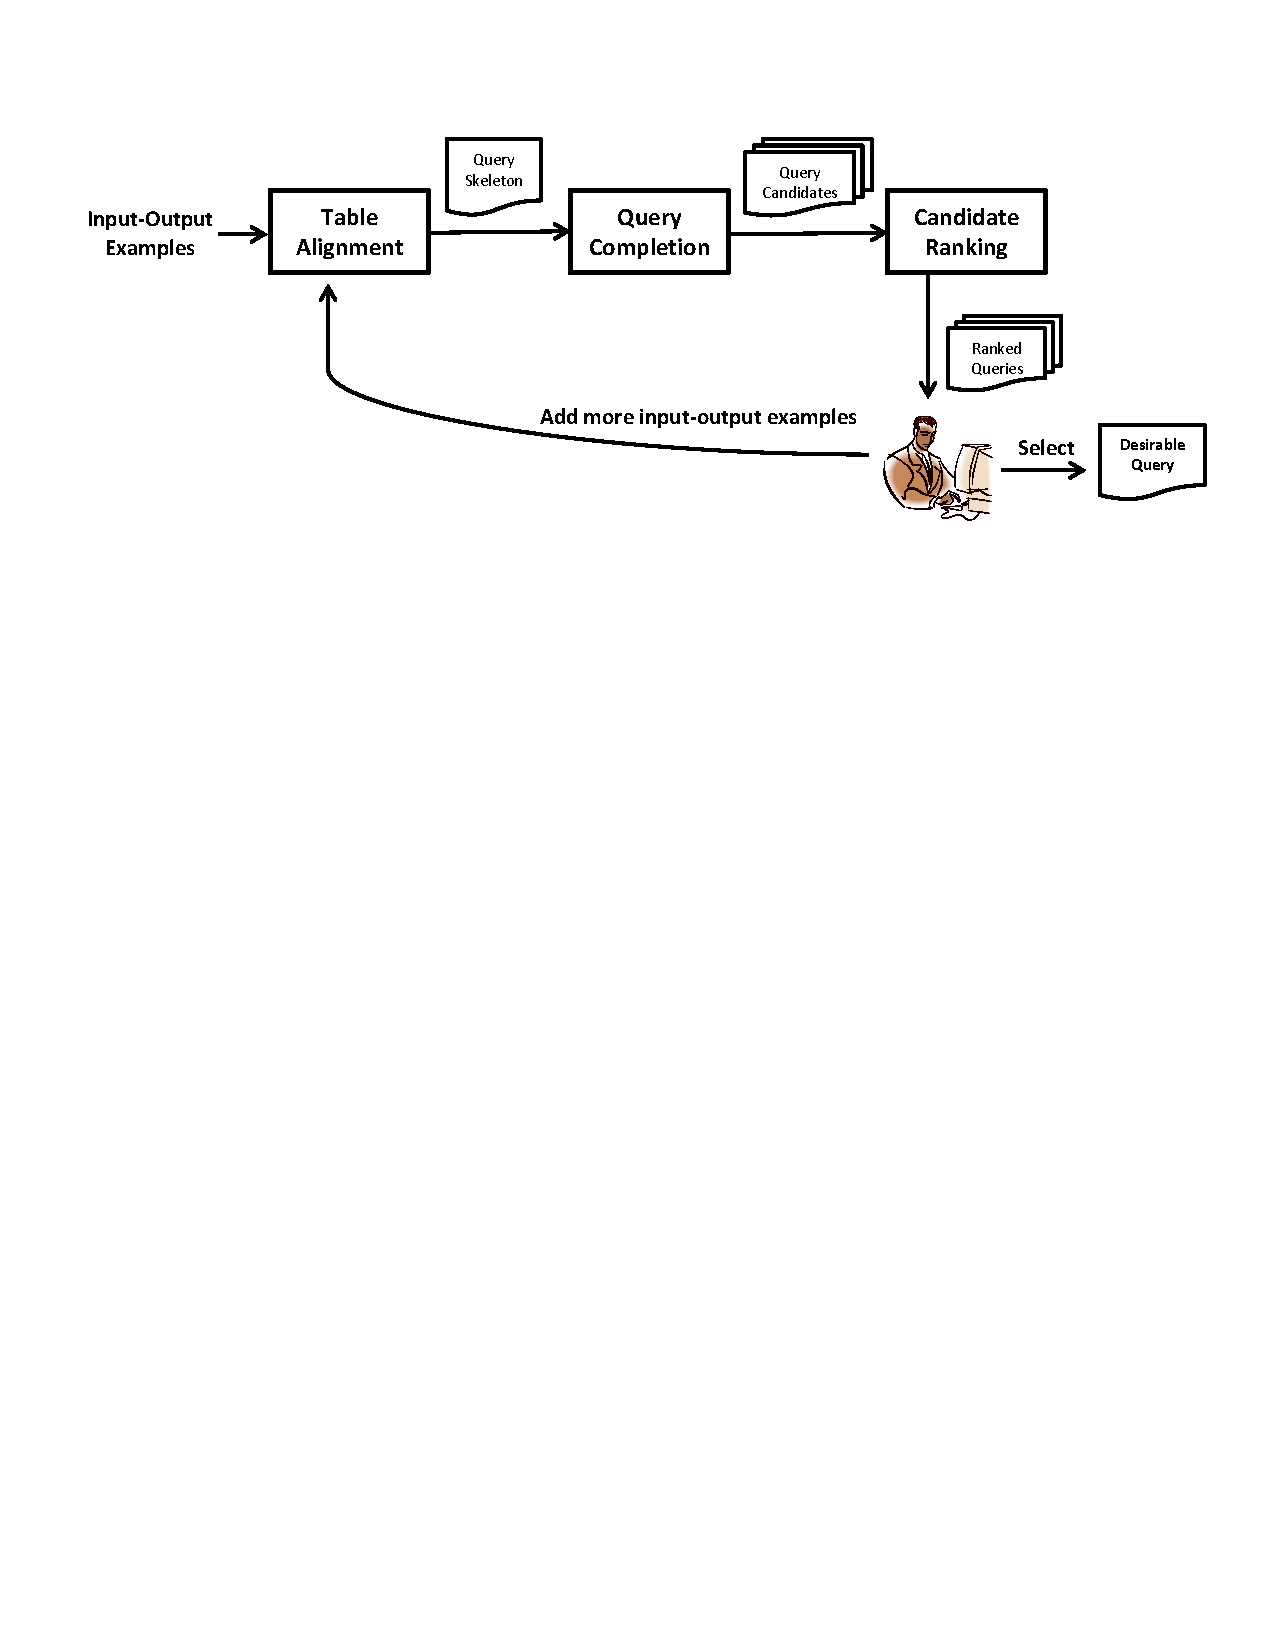
\includegraphics[scale=0.46]{workflow}
  \vspace*{-5.0ex}\caption {{\label{fig:workflow} The workflow of our SQL synthesis tool.
}}
\end{figure}

Our tool takes as input a pair of input-output examples. It first performs
table alignment to infer a partially complete query skeleton. The inferred query
skeleton, which contains unknown parts as holes, is not a valid SQL query.
In the next step, our tool uses the search strategy as defined in Section~\ref{sec:completion}
to complete this partial query, and produces a list of query candidates.
A query candidate is a valid, complete SQL query statement which satisfies
the provided input-output example. However, for a realistic problem,
multiple query candidates can be generated. The tool next ranks the candidate
query list, and provides users a ranked list of SQL queries with the most likely
ones on the top.

This tool also takes the user interaction model (Section~\ref{sec:uim}) into account.
The user could either select a desirable query from the output ranked list, or provide
the tool additional examples to infer more accurate queries.

In our implementation, we choose MySQL as the backend database engine, which takes an
inferred SQL query candidate, executes it on the input tables, and checks whether the
result match the given output example.

\sai{wrote in more details}
